\documentclass[12pt,a4paper]{article}
\usepackage{amsmath,amssymb}
\usepackage{graphicx}
\usepackage{float}
\usepackage{tikz}
\usetikzlibrary{shapes, arrows, positioning}


\usepackage{amsmath,amssymb,mdframed}            % AMS package gives better equation layouts
\setcounter{page}{5}                    % sets first page number to 2
\setlength{\oddsidemargin}{-0.25in}     % set left margin
\setlength{\textwidth}{6.5in}           % set text width
\setlength{\topmargin}{-0.5in}          % controls layout at
\setlength{\headsep}{0.5in}             % top of page
\setlength{\textheight}{9.0in}          % set text length



\makeatletter
\renewcommand{\@oddhead}{\hfill MA3600/Mock-solution}  % sets header
\renewcommand{\@oddfoot}{\hfil \arabic{page} \hfil}    % sets page footer
\makeatother

\renewcommand{\labelenumi}{\arabic{enumi}} % Sets the first level of enumerate to be arabic (normal) numbers
\renewcommand{\labelenumii}{(\alph{enumii})} %Sets the second level of enumerate to be (a), (b), (c), .....
\renewcommand{\labelenumiii}{(\roman{enumiii})} % Sets the third level of enumerate to be (i), (ii), (iii), ....



\begin{document}
\null \vskip1cm
\begin{enumerate}
\setcounter{enumi}{3}

\renewcommand\labelenumi{\bfseries\theenumi.}

\item

    \begin{enumerate}
        \item Provide definitions for the following terms:
            \begin{itemize}
                \item Normal form game.\\


                A $N$ player \textbf{normal form game} consists of:
                \begin{itemize}
                \item A finite set of $N$ players;
                \item Strategy spaces for the players: $S_1, S_2, S_3, \dots S_N$;
                \item Payoff functions for the players: $u_i:S_{1}\times S_2\dots\times S_N\to \mathbb{R}$
                \end{itemize}

                ~\hfill{[1]}

                \item Strictly dominated strategy.\\

                In an $N$ player normal form game. A pure strategy $s_i\in S_i$ is said to be \textbf{strictly dominated} if there is a strategy $\sigma_i\in \Delta S_i$ such that $u_i(\sigma_i,s_{-i})>u_{i}(s_i,s_{-i})$ for all $s_{-i}\in S_{-i}$ of the other players.

                ~\hfill{[1]}

                \item Weakly dominated strategy.\\

                In an $N$ player normal form game. A pure strategy $s_i\in S_i$ is said to be \textbf{weakly dominated} if there is a strategy $\sigma_i\in \Delta S_i$ such that $u_i(\sigma_i,s_{-i})\geq u_{i}(s_i,s_{-i})$ for all $s_{-i}\in S_{-i}$ of the other players and there exists a strategy profile $\bar s\in S_{-i}$ such that $u_i(\sigma_i,\bar s)> u_{i}(s_i,s_{-i})$ .
                ~\hfill{[1]}

                \item Best response strategy.\\

                In an $N$ player normal form game. A strategy $s^*$ for player $i$ is a best response to some strategy profile $s_{-i}$ if and only if $u_i(s^*,s_{-i})\geq u_{i}(s,s_{-i})$ for all $s\in S_i$.
                ~\hfill{[1]}

                \item Nash equilibrium.\\

                In an $N$ player normal form game. A Nash equilibrium is a strategy profile $\tau = (\tilde s_1,\tilde s_2,\dots,\tilde s_N)$ such that:

                $$u_i(\tilde s)\geq u_i(\bar s_i,\tilde s_{-i})\text{ for all }i$$
                ~\hfill{[1]}
            \end{itemize}

        For the remainder of this question consider the battle of the sexes game:

            \[\begin{pmatrix}
            (1,-1) & (-2,2)\\
            (-3,3) & (1,-1)\\
            \end{pmatrix}\]

        \item By clearly stating the techniques used: obtain all (if any) pure Nash equilibrium.

            We attempt to identify best responses under the assumption of common knowledge of rationality:

            \[\begin{pmatrix}
            (\underline{1},-1) & (-2,\underline{2})\\
            (-3,\underline{3}) & (\underline{1},-1)\\
            \end{pmatrix}\]

            There is no pure Nash equilibrium.

        ~\hfill{[4]}

        \item Plot the utilities to player 1 (the row player) assuming that the 2nd player (the column player) plays a mixed strategy: $\sigma_2 = (y,1-y)$.

        We have:

        $$u_1(r_1,\sigma_2)=y-2+2y=3y-2$$

        and

        $$u_1(r_2,\sigma_2)=-3y+1-y=1-4y$$

        ~\hfill{[1]}

        Which gives:

        \begin{center}
            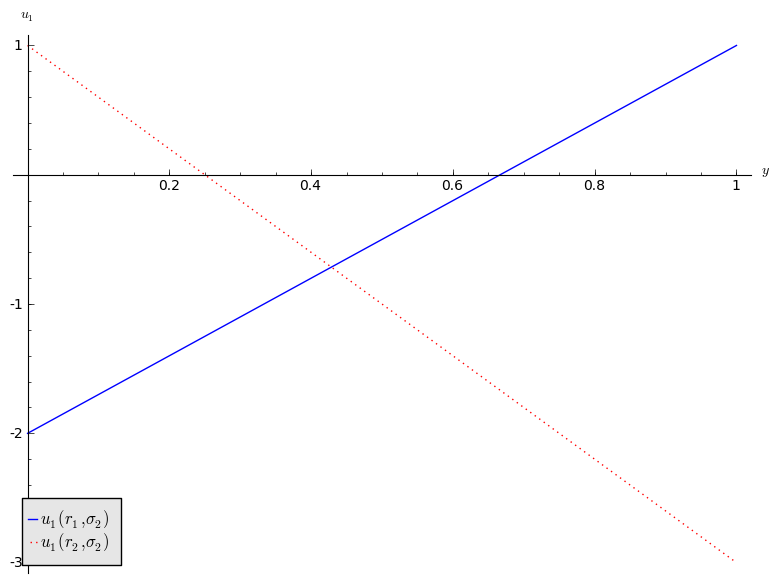
\includegraphics[width=.5\textwidth]{./plots/mock-plt01.png}
        \end{center}

        ~\hfill{[1]}

        \item Plot the utilities to player 2 (the column player) assuming that the 1st player (the row player) plays a mixed strategy: $\sigma_1 = (x,1-x)$.

        We have:

        $$u_2(\sigma_1,s_1)=-x+3-3x=3-4x$$

        and

        $$u_2(\sigma_1,s_2)=2x-1+x=3x-1$$

        ~\hfill{[1]}

        Which gives:

        \begin{center}
            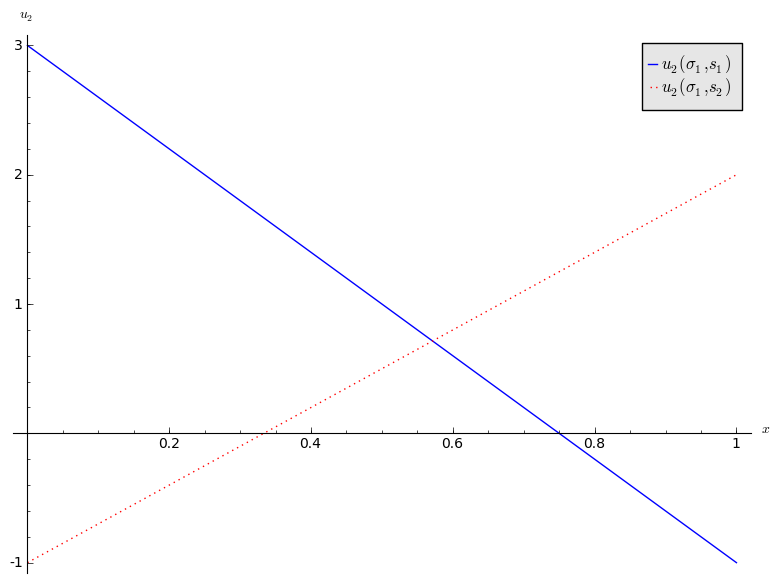
\includegraphics[width=.5\textwidth]{./plots/mock-plt02.png}
        \end{center}

        ~\hfill{[1]}

        \item Assuming that player 1 plays the mixed strategy $\sigma_1=(x,1-x)$, show that player 1's best response $x^*$ to a mixed strategy $\sigma_2 = (y,1-y)$ is given by:


            \[
            x^*=\begin{cases}
                0,&\text{ if } y < 3/7\\
                1,&\text{ if } y > 3/7\\
                \text{indifferent},&\text{ otherwise }\\
            \end{cases}
            \]

            We have $u_1(r_2,\sigma_2)=u_1(r_1,\sigma_2)$ $\Rightarrow$ $y=3/7$. From the plots we see that if $y<3/7$ then player 1's best response is to play $r_2$ which corresponds to $x=0$, similarly for $y>3/7$ and finally if $y=3/7$ player 1 is indifferent.

        ~\hfill{[2]}

            Similarly show that player 2's best response $y^*$ is given by:

            \[
            y^*=\begin{cases}
                0,&\text{ if } x < 4/7\\
                1,&\text{ if } x > 4/7\\
                \text{indifferent},&\text{ otherwise }\\
            \end{cases}
            \]

            We have $u_2(\sigma_1,s_1)=u_1(\sigma_1,s_2)$ $\Rightarrow$ $x=4/7$. From the plots we see that if $x<4/7$ then player 2's best response is to play $s_1$ which corresponds to $y=1$, similarly for $x>4/7$ and finally if $x=4/7$ player 2 is indifferent.

        ~\hfill{[2]}

        \item Use the above to obtain all Nash equilibria for the game.

        We see that the only mixed strategy that is a pair of best responses is $(\sigma_1,\sigma_2)=((4/7,3/7),(3/7,4/7))$.
        ~\hfill{[2]}

        \item Confirm this result by stating, proving and using the Equality of Payoffs theorem.

            The equality of payoffs theorem states:

            In an $N$ player normal form game if the strategy profile $(\sigma_i,s_{-i})$ is a Nash equilibria then:

            $$u_{i}(\sigma_i,s_{-i})=u_{i}(s,s_{-i})\text{ for all }s\in\mathcal{S}(\sigma_i)\text{ for all }1\leq i\leq N$$

            ~\hfill{[1]}

            \textbf{Proof:}

            If $|\mathcal{S}(\sigma_i)|=1$ then the proof is trivial.

            We assume that $|\mathcal{S}(\sigma_i)|>1$. Let us assume that the theorem is not true so that there exists $\bar s\in\mathcal{S}(\sigma)$ such that

            $$u_{i}(\sigma_i,s_{-i})\ne u_{i}(\bar s,s_{-i})$$

            Without loss of generality let us assume that:

            $$\bar s=\text{argmax}_{s\in\mathcal{S}(\sigma)}u_i(s,s_{-i})$$

            Thus we have:

            $$\begin{aligned}
            u_i(\sigma_i,s_{-i})&=\sum_{s\in\mathcal{S}(\sigma_i)}\sigma_i(s)u(s,s_{-i})\\
            &\leq \sum_{s\in\mathcal{S}(\sigma_i)}\sigma_i(s)u(\bar s,s_{-i})\\
            &\leq u(\bar s,s_{-i})\sum_{s\in\mathcal{S}(\sigma_i)}\sigma_i(s)\\
            &\leq u(\bar s,s_{-i})\\
            \end{aligned}$$

            Giving:

            $$u_{i}(\sigma_i,s_{-i})< u_{i}(\bar s,s_{-i})$$

            which implies that $(\sigma_i,s_{-i})$ is not a Nash equilibrium.

            ~\hfill{[4]}

            To verify the mixed Nash equilibria found previously we apply the theorem:

            $$u_1(r_1,\sigma_2)=u_1(r_2,\sigma_2)\Rightarrow \tilde y=3/7$$
            $$u_2(\sigma_1, s_1)=u_2(\sigma_1, s_2)\Rightarrow \tilde x=4/7$$

            As required.

            ~\hfill{[1]}


    \end{enumerate}

\newpage
\item

    \begin{enumerate}

            \item Consider the centipede game shown below:

            \begin{center}
                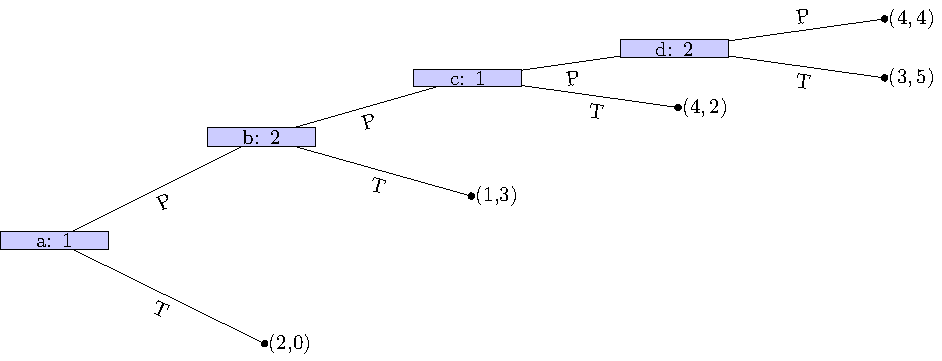
\includegraphics[width=.8\textwidth]{images/mock-img01.pdf}
            \end{center}

            Obtain a subgame perfect Nash equilibrium for this game (you are expected to prove that it is a subgame perfect Nash equilibrium).

            Writing down the normal form representation of the game gives the following two strategy sets:

            \[S_1=\{PP,PT,TP,TT\}\]
            \[S_2=\{PP,PT,TP,TT\}\]

            \hfill[2]

            Using that ordering of strategies the normal form representation of the game is given with the best responses shown:

            \[\begin{pmatrix}
            (\underline{4},4)&(3,\underline{5})&(1,3)&(1,3)\\
            (\underline{4},2)&(\underline{4},2)&(1,\underline{3})&(1,\underline{3})\\
            (2,\underline{0})&(2,\underline{0})&(\underline{2},\underline{0})&(\underline{2},\underline{0})\\
            (2,\underline{0})&(2,\underline{0})&(\underline{2},\underline{0})&(\underline{2},\underline{0})\\
            \end{pmatrix}\]

            \hfill[4]

            This identifies 4 pure Nash equilibria: \(\{(TP,TP),(TP,TT),(TT,TP),(TT,TT)\}\).

            \hfill[1]

            If we consider the subgame generated by node b then all 4 are still Nash equilbria.

            \hfill[1]

            If we consider the subgame generated by node c then only \(TT,TT\) is a Nash equilibria which is also a Nash equilibria for the subgame generated by node d.

            \hfill[2]

            Thus \((TT,TT)\) is a the only subgame perfect Nash equilibria.

            \hfill[1]


            \item Prove the following theorem:

            ``For any finitely repeated game, any sequence of stage Nash profiles gives the outcome of a subgame perfect Nash equilibrium.''

            \hfill[4]

            If we consider the strategy given by:

            ``Player $i$ should play strategy $\tilde s^{(k)}_i$ regardless of the play of any previous strategy profiles."

            where $\tilde s^{(k)}_i$ is the strategy played by player $i$ in any stage Nash profile. The $k$ is used to indicate that all players play strategies from the same stage Nash profile.

            Using backwards induction we see that this strategy is a Nash equilibrium. Furthermore it is a stage Nash profile so it is a Nash equilibria for the last stage game which is the last subgame. If we consider (in an inductive way) each subsequent subgame the result holds.

            \item If they exist identify all subgame perfect Nash equilibrium for the following two games:

                \begin{center}
                    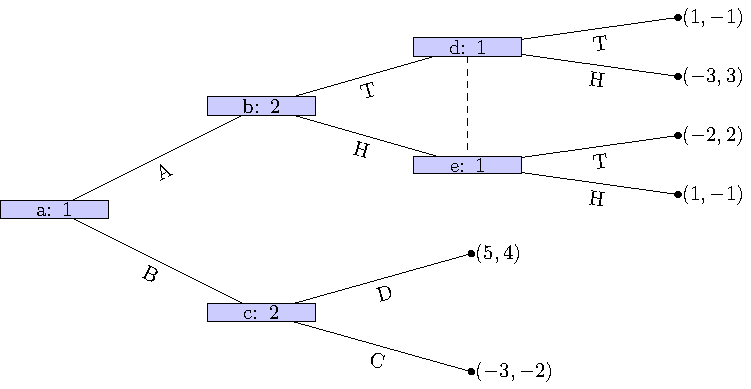
\includegraphics[width=.8\textwidth]{images/mock-img02.pdf}\\
                \end{center}

                The strategy sets are:

                \[S_1=\{AT,AH,BT,BH\}\]
                \[S_2=\{TD,TC,HD,HC\}\]

                \hfill[2]

                This gives the following normal form representation (with best responses shown):

                \[\begin{pmatrix}
                (\underline{1},-1)&(\underline{1},-1)&(-2,\underline{2})&(-2,\underline{2})\\
                (-3,\underline{3})&(-3,\underline{3})&(\underline{1},-1)&(\underline{1},-1)\\
                (\underline{5},\underline{4})&(-3,-2)&(\underline{5},\underline{4})&(-3,-2)\\
                (\underline{5},\underline{4})&(-3,-2)&(\underline{5},\underline{4})&(-3,-2)\\
                \end{pmatrix}\]

                \hfill[2]

                We have 4 pure Nash equilibrium: \((BT,TD),(BT,HD),(BH,TD),(BH,HD)\).

                \hfill[1]

                Considering the subgame generated by node b (using \(S_1=\{BT,BH\}\) and \(S_2=\{TD,HD\}\)):

                \[
                \begin{pmatrix}
                (1,-1)&(-2,2)\\
                (-3,3)&(1,-1)\\
                \end{pmatrix}
                \]

                \hfill[1]

                by the equality of payoffs theorem the mixed Nash equilibrium \((x,1-x),(y,1-y)\) is a solution to:

                \[y-2+2y=-3y+1-y\]
                \[-x+3-3x=2x-1+x\]

                \hfill[1]

                which gives \(x=4/7\) and \(y=3/7\) thus the only subgame perfect Nash equilibrium is:

                \[(0,0,4/7,3/7),(3/7,0,4/7,0)\]

                \hfill[1]

                \begin{center}
                    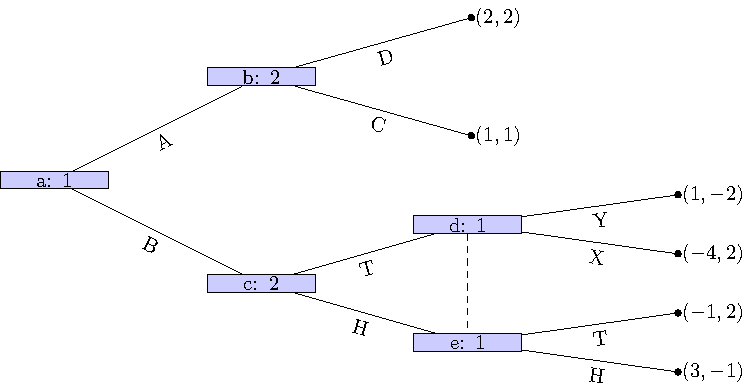
\includegraphics[width=.8\textwidth]{images/mock-img03.pdf}
                \end{center}

                This is not a valid game as the strategies available in the information set containing nodes d and e are not the same.

                \hfill[2]

    \end{enumerate}

\newpage
\item


    \begin{enumerate}

        \item Define a stochastic game.

            A stochastic game is defined by:

            \begin{itemize}
            \item X a set of states with a stage game defined for each state;
            \item A set of strategies $S_i(x)$ for each player for each state $x\in X$;
            \item A set of rewards dependant on the state and the actions of the other players: $u_i(x,s_1,s_2)$;
            \item A set of probabilities of transitioning to a future state: $\pi(x'|x,s_1,s_2)$;
            \item Each stage game is played at a set of discrete times $t$.
            \end{itemize}

        \hfill[4]

        \item Define a Markov strategy.

            A strategy is call a Markov strategy if the behaviour dictated is not time dependent.

        \hfill[2]

        \item Give the conditions for Nash equilibrium in a stochastic game.

            A Nash equilibrium satisfies:

            $$U_1^*(x)=\max_{r\in S_1(x)}(u_i(x,r,s^*)+\delta\sum_{x'\in X}\pi(x'|x,r,s^*)U_1^*(x')$$
            $$U_2^*(x)=\max_{s\in S_2(x)}(u_i(x,r^*,s)+\delta\sum_{x'\in X}\pi(x'|x,r^*,s)U_1^*(x')$$

        \hfill[3]

        \item Obtain the pure strategy Nash equilibria (if it exists) for the following game with \(\delta=.5\):

        \begin{center}
            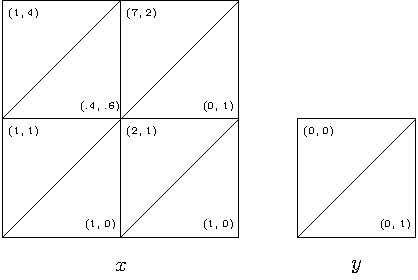
\includegraphics[width=.8\textwidth]{images/mock-img04.pdf}
        \end{center}

        State \(y\) gives no value to either player so we only need to consider state \(x\). Let the future gains to 1 in state \(x\) by \(u\) and the future gains to player 2 in state \(x\) be \(v\). Thus the players are facing the following game:

        \hfill[2]

        \[\begin{pmatrix}
        (1+1/5u,4+1/5v)&(7,2)\\
        (1+1/2u,1+1/2v)&(2+1/2u,1+1/2v)
        \end{pmatrix}\]

        \hfill[2]

        There are 4 potential pure strategy equilibrium:

        \begin{itemize}
            \item \((a,c)\) which requires \(1+1/5u\geq1+1/2u\) and \(4+1/5v\geq2\) \(\Rightarrow\) \(u\leq 0\) and \(v\geq -10\). If this is the equilibria then \(u=1+1/5u\) which gives \(u=5/4\) which contradicts the constraint.
            \hfill[3]
            \item \((a,d)\) which requires \(7\geq2+1/2u\) and \(4+1/5v\leq2\) \(\Rightarrow\) \(u\leq 10\) and \(v\leq -10\). If this is the equilibria then \(v=2\) which contradicts the constraint.
            \hfill[3]
            \item \((b,c)\) which requires \(1+1/5u\leq1+1/2u\) and \(1+1/2v\geq1+1/2v\) \(\Rightarrow\) \(u\geq 0\). If this is the equilibria then \(u=2\) and \(v=2\) which contradicts no constraints.
            \hfill[3]
            \item \((b,d)\) which requires \(2+1/2u\geq 7\) and \(1+1/2v\geq1+1/2v\) \(\Rightarrow\) \(u\geq 10\). If this is the equilibria then \(u=2\) which contradicts the constraints.
            \hfill[3]
        \end{itemize}

        Thus \((b,c)\) is the unique Nash Equilibrium.


    \end{enumerate}
\end{enumerate}


\makeatletter
\renewcommand{\@oddfoot}{\hfil \arabic{page}X \hfil}    % sets last page footer
\makeatother

\end{document}
